\documentclass{article}
\usepackage{array}
\usepackage[column=0]{cellspace}
\setlength\cellspacetoplimit{6pt}
\setlength\cellspacebottomlimit{6pt}
\usepackage{graphicx} % Required for inserting images
\usepackage{amsmath}
\usepackage{amssymb}
\usepackage{amsthm}
\usepackage{amsfonts}
\usepackage{gensymb}
\newcommand{\myvec}[1]{\ensuremath{\begin{pmatrix}#1\end{pmatrix}}}
\usepackage{graphicx}
\usepackage{amsmath}
\usepackage{mathtools}
\usepackage{gensymb}

\newcommand{\mydet}[1]{\ensuremath{\begin{vmatrix}#1\end{vmatrix}}}
\providecommand{\brak}[1]{\ensuremath{\left(#1\right)}}
\providecommand{\norm}[1]{\left\lVert#1\right\rVert}
\newcommand{\solution}{\noindent \textbf{Solution: }}
\let\vec\mathbf

\title{MathConstruction}

\begin{document}

\section{NCERT 12.10.5.9}

Find the position vector of a point C which divides the line joining two points A and B whose Position Vectors are $2\overrightarrow{a}+\overrightarrow{b}$ and $\overrightarrow{a}-3\overrightarrow{b}$ externally in the ration $1:2$.Also, Show that A is the mid point of the line segment BC \\
\textbf{Solution:}
The coordinates and ratio are given as
\begin{align}
\vec{A}=\myvec{2\\1\\},
\vec{B}=\myvec{1\\-3\\},
n=\frac{2}{1}
\end{align}
Using section formula
\begin{align}
    \vec{C}=\frac{B-n.A}{1-n}\\
    \vec{C}=\frac{\myvec{1\\-3}-2.\myvec{2\\1}}{1-2}\\
    \vec{C}=\myvec{3\\5}
\end{align}
\begin{enumerate}
    \begin{figure}[!ht]
       \centering
       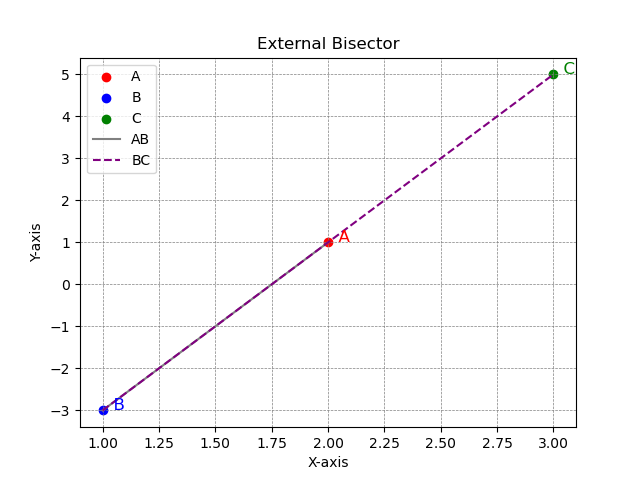
\includegraphics[width=\columnwidth]{/sdcard/geometry/codes/external_bisector.png}
       \caption{point vectors A,B,C}
       \label{fig:enter-label}
    \end{figure}
\end{enumerate}
\end{document}
